\documentclass[Report.tex]{subfiles}

% Read data
%\pgfplotstableread[col sep=comma]{results/feature_eval_ratio.csv}\evalratio

\begin{document}

%\newcommand{\accprerecbarplot} {
%  \addplot+[
%    discard if not={feature}{#1},
%] table [x expr=\coordindex, y={accuracy}] {};
%}
\section{Experiments}
This section describes the different experiments conducted and analyses their results. For all experiments, the dataset is split into training and testing data. When splitting the dataset for pair classification TODO section, no players in the training set appear in the testing set. All experiments used a two-step evaluation method to obtain metrics for training and testing.
\begin{enumerate}
\item During training, evaluation metrics were gathered using a 5-fold cross evaluation. This gives an idea on how well the models and feature perform, but the performance is likely inflated as the same player may appear in both the training and evaluation data. 
\item After the 5-fold cross evaluation, the final model is trained using all the training data, and evaluated against the testing data. This is the best indication of how the models perform against unseen data, as the testing data is untouched until this point of the experiment. 
\end{enumerate}

\subsection{Mouse movement features}
The first experiments and results run looked only at using the mouse movement features to see how effective they were at predicting the player. As there are three types of mouse movement feature (MMAC, MMMC and MMSC) as described in section \ref{sec:mm-features}, each feature is first evaluated individually, to see which feature may be more important to player prediction. 
\begin{figure}[H]
\begin{subfigure}{0.45\textwidth}
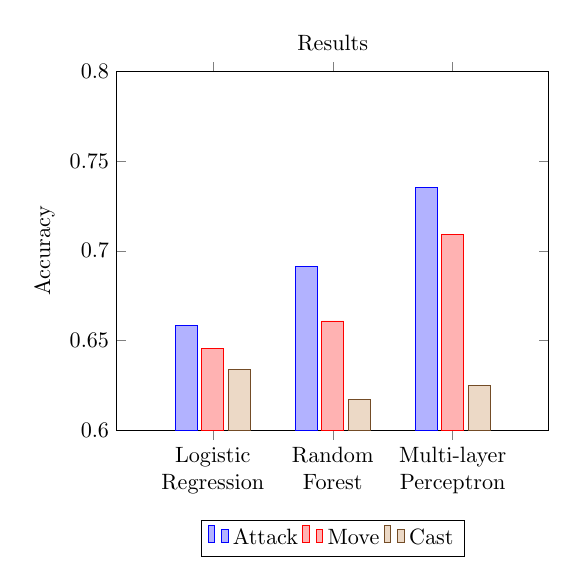
\begin{tikzpicture}[scale=0.8]
\begin{axis}[
    ybar,
    title={Results},
    ymin=0.6, ymax=0.8,
    bar width=1em,
    legend style={at={(0.5,-0.25)},anchor=north,legend columns=-1},
    enlarge x limits=0.4,
    x tick label style={align=center,text width=1.7cm},
    symbolic x coords={Logistic Regression, Random Forest, Multi-layer Perceptron},
    xtick=data,
    ylabel={Accuracy}
]
  \addplot coordinates {(Logistic Regression,0.6586) (Random Forest,0.6915) (Multi-layer Perceptron,0.7355)};
  \addplot coordinates {(Logistic Regression,0.6457) (Random Forest,0.6609) (Multi-layer Perceptron,0.7094)};
  \addplot coordinates {(Logistic Regression,0.6339) (Random Forest,0.6173) (Multi-layer Perceptron,0.6248)};
\legend{Attack,Move,Cast}

\end{axis}
\end{tikzpicture}
\end{subfigure}
\hspace{\fill}
\begin{subfigure}{0.45\textwidth}
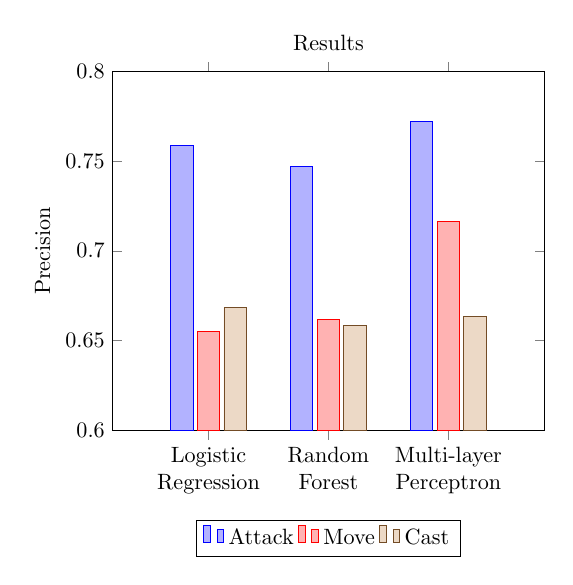
\begin{tikzpicture}[scale=0.8]
\begin{axis}[
    ybar,
    title={Results},
    ymin=0.6, ymax=0.8,
    bar width=1em,
    legend style={at={(0.5,-0.25)},anchor=north,legend columns=-1},
    enlarge x limits=0.4,
    x tick label style={align=center,text width=1.7cm},
    symbolic x coords={Logistic Regression, Random Forest, Multi-layer Perceptron},
    xtick=data,
    ylabel={Precision}
]
  \addplot coordinates {(Logistic Regression,0.759) (Random Forest,0.747) (Multi-layer Perceptron,0.7719)};
  \addplot coordinates {(Logistic Regression,0.65524) (Random Forest,0.6618) (Multi-layer Perceptron,0.7165)};
  \addplot coordinates {(Logistic Regression,0.6683) (Random Forest,0.6582) (Multi-layer Perceptron,0.6633)};
\legend{Attack,Move,Cast}
\end{axis}
\end{tikzpicture}
\end{subfigure}
\caption{Classification rates using only mouse movement features.}
\label{fig:move-results}
\end{figure}


%\begin{tikzpicture}
%\begin{axis}[
%    ybar,
%    title={Results},
%    bar width=1em,
%    legend style={at={(0.5,-0.25)},
%      anchor=north,legend columns=-1},
%    enlarge x limits=0.4,
%
%    x tick label style={align=center,text width=1.7cm},
%    symbolic x coords={Logistic Regression, Random Forest, Multi-layer Perceptron},
%    xtick=data,
%    ylabel={Recall}
%]
%  \addplot coordinates {(Logistic Regression,0.6747) (Random Forest,0.7754) (Multi-layer Perceptron,0.8243)};
%  \addplot coordinates {(Logistic Regression,0.672) (Random Forest,0.6975) (Multi-layer Perceptron,0.7239)};
%  \addplot coordinates {(Logistic Regression,0.6665) (Random Forest,0.6301) (Multi-layer Perceptron,0.6909)};
%\legend{Attack,Move,Cast}
%\end{axis}
%\end{tikzpicture}

\subsection{Game statistic features}

\subsection{Game itemisation features}

\subsection{Combining features}

\end{document}
